\documentclass{../exhibit}

\title{Pirate Queens}

%% Font
\usepackage{imfellEnglish}
\usepackage[T1]{fontenc}
\raggedright

\usepackage{background}

\backgroundsetup{
scale=1,
color=black,
opacity=0.4,
angle=0,
contents={%
  \includegraphics[height=\paperheight]{mapBackground.jpg}%%https://upload.wikimedia.org/wikipedia/commons/8/81/Nautical_chart_of_the_West_Indies_1797.jpg
  }%
}




%% For the context
%% https://tex.stackexchange.com/questions/86150/torn-page-effect/86151#86151
\usepackage{tikz}
\usetikzlibrary{decorations.pathmorphing}
\definecolor{paper}{RGB}{239,227,157}





\renewcommand{\maketitle}{ %
  \begin{center}
    \scalebox{8}{\thetitle}
  \end{center}
  
\begin{tabular*}{\textwidth}{c @{\extracolsep{\fill}} c}  
\resizebox{4in}{!}{\begin{minipage}[b]{3in}\huge\directions\end{minipage}} &
  \resizebox{4in}{!}{
\begin{tikzpicture}[pencildraw/.style={ %
    decorate,
    decoration={random steps,segment length=4pt,amplitude=2pt}
    } %
]
\node[
preaction={fill=black,opacity=.5,transform canvas={xshift=.5cm,yshift=-.5cm}},
pencildraw,draw,fill=paper,text width=3in,inner sep=.5cm] 
{\begin{center}\Huge Capt'n Gauss' log \end{center}\vspace{.7cm} {\huge\context}};
\end{tikzpicture}}

\end{tabular*}

\vfill

\includegraphics[width=3in]{logoPirate.png}\hfill \includegraphics[width=2in]{bammLogo.png}


}


\begin{document}



\begin{context}
  Pirates be a suspicious bunch!


  The Pirate Queen known as Noether be no different!


  When in the rooms, she insists that her crew, queens all of them, take the room!

    
  Show how these pirate queens must stand to dominate their land!
\end{context}



\begin{directions}
  Take a $n\ x\ n$ chessboard. How many queens can you place so that
  none are attacking the others?
\end{directions}



\begin{example}
 If $4$ Pirate Queens in a room of $4x4$, how could they stand?
\begin{center}
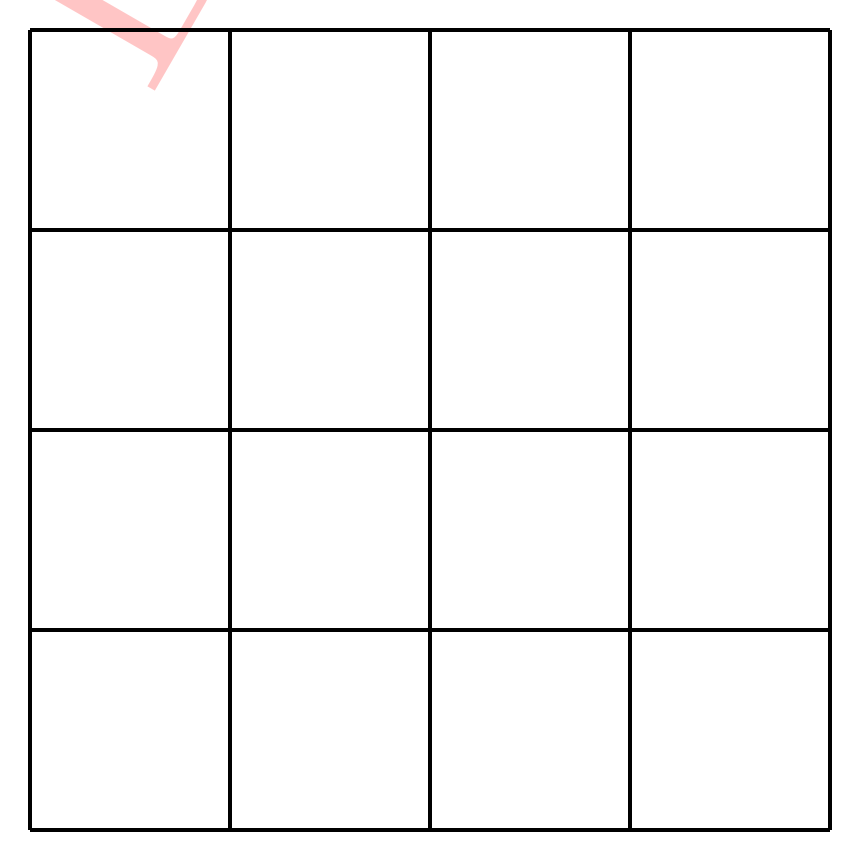
\begin{tikzpicture}
\draw[step=1in,ultra thick] (0,0) grid (4in,4in);
\node at (1.5in,3.5in) {\scalebox{2}{\BlackQueenOnWhite}};
\node at (.5in,1.5in) {\scalebox{2}{\BlackQueenOnWhite}};
\node at (2.5in,.5in) {\scalebox{2}{\BlackQueenOnWhite}};
\node at (3.5in,2.5in) {\scalebox{2}{\BlackQueenOnWhite}};
\end{tikzpicture}
\end{center}
\end{example}



\begin{mathConnections}
  https://bartsnapp.github.io/Math-Outreach-Exhibits/chess/
\end{mathConnections}
\end{document}
